\documentclass[11pt]{article}
\usepackage{amsmath}
\usepackage{amssymb}
\usepackage{amsthm}
\usepackage{caption}
\usepackage{cleveref}
\usepackage{enumitem}
\usepackage{graphicx}
\usepackage[totalwidth=480pt, totalheight=680pt]{geometry}
\usepackage{mathrsfs}
\usepackage{tikz}
\usetikzlibrary{calc}
\usepackage{xcolor}
\usepackage[round]{natbib}
\definecolor{mid_green}{HTML}{99d8c9}

\captionsetup{width=0.8\textwidth}
\DeclareMathOperator*{\argmax}{arg\,max}
\newtheorem{definition}{Definition}
\newtheorem{lemma}{Lemma}
\newtheorem{theorem}{Theorem}
\setlength{\tabcolsep}{1em}
\setlist{listparindent=\parindent, parsep=0pt}

\newcommand{\EE}{\mathbb{E}}
\newcommand{\PP}{\mathbb{P}}
\newcommand{\RR}{\mathbb{R}}

% Commands for inline commenting that shows up on pdf
\newcommand{\WFcomment}[1]{{\color{red}{(WF: \bf \sc #1) }}}
\newcommand{\KHcomment}[1]{{\color{green!60!black}{(KH: \bf \sc #1) }}}

\begin{document}

\title{Rank verification for exponential families}
\author{Kenneth Hung \and William Fithian}
\date{\today}
\maketitle

\begin{abstract}
Many statistical experiments involve comparing multiple population groups. For example, a public opinion poll may ask which of several political candidates commands the most support, or a clinical trial may compare patient outcomes to determine the best of several treatment conditions. This article concerns the problem of {\em rank verification} --- post hoc tests of whether the ordering discovered in the data is in fact statistically significant. For exponential family models, we show under mild conditions that an unadjusted two-tailed pairwise test comparing the ``winning'' population to the ``runner-up'' is a valid test of whether the winner is truly the best. We also propose comparably simple procedures to give lower confidence bounds on the gap between the winning population and the others, and to verify ranks beyond the first.
\end{abstract}

\section{Introduction}
\label{sec:introduction}

\subsection{Motivating Example: Iowa Republican Caucus Poll}\label{sec:iowa}

Table~\ref{tbl:poll} shows the result of a Quinnipiac University poll asking 890 Iowa Republicans their preferred candidate for the Republican presidential nomination \citep{quinnipiac}. Donald Trump led with $31\%$ of the vote, Ted Cruz came second with $24\%$, Marco Rubio third with $17\%$, and ten other candidates including ``Don't know'' trailed behind. 

\begin{table}[htbp]
\begin{center}
\begin{tabular}{c c c c}
	\hline
	Rank & Candidate & Result & Votes \\
	\hline
	$1$ * & Trump & $31\%$ & $276$ \\
	$2$ * & Cruz & $24\%$ & $214$ \\
	$3$ * & Rubio & $17\%$ & $151$ \\
	$4$ * & Carson & $8\%$ & $71$ \\
	$5$ & Paul & $4\%$ & $36$ \\
	$6$ & Bush & $4\%$ & $36$ \\
	$7$ & Huckabee & $3\%$ & $27$ \\
	$\vdots$ & $\vdots$ & $\vdots $ & $\vdots$ \\
	\hline
\end{tabular}
\end{center}
\caption{Results from a February 1, 2016 Quinnipiac University poll of $890$ Iowa Republicans. To compute the last column (Votes), we make the simplifying assumption that the reported percentages in the third column (Result) correspond to raw vote shares among survey respondents. The asterisks indicate that the rank is verified through a step-down procedure.}
\label{tbl:poll}
\end{table}

Seeing that Trump leads this poll, several salient questions may occur to us: Is Trump really winning, and if so by how much? And analogously, is Cruz really in second, is Rubio really in third, and so on? Note that there is implicitly a problem of multiple comparisons here, because if Cruz had led the poll instead, we would be asking a different set of questions. Indeed, the selection issue appears especially pernicious due to the so-called ``winner's curse:'' given that Trump leads the poll, it more likely than not overestimates his support.

Nevertheless, if we blithely ignore the selection issue, we might carry out the following analyses to answer the questions we posed before at significance level $\alpha=0.05$. We assume for simplicity that the poll represents a simple random sample of Iowa Republicans, i.e., that the data are a multinomial sample of size $890$ and underlying probabilities $(\pi_{\text{Trump}}, \pi_{\text{Cruz}}, \ldots)$.\footnote{The reality is a bit more complicated: before releasing the data, Quinnipiac has processed it to make the reported result more representative of likely caucus-goers.}
\begin{enumerate}
\item {\em Is Trump really winning?} If Trump and Cruz were in fact tied, then Trump's share of their combined 490 votes would be distributed as $\text{Binom}(490, 0.5)$. Because the (two-tailed) $p$-value for this pairwise test is $p=0.006$, we reject the null and conclude that Trump is really winning.
\item {\em By how much?} Using an exact $95\%$ interval for the same binomial model, we conclude Trump has at least $7.5\%$ more support than Cruz (i.e., $\pi_{\text{Trump}} \geq 1.075 \,\pi_{\text{Cruz}}$) and also leads the other candidates by at least as much.
\item {\em Is Cruz in second, Rubio in third, etc.?} We can next compare Cruz to Rubio just as we compared Trump to Cruz (again rejecting because 214 is significantly more than half of 365), then Rubio to Carson, and so on, continuing until we fail to reject. The first four comparisons are all significant at level $0.05$, but Paul and Bush are tied so we stop.
\end{enumerate}

Surprisingly, all of the three procedures described above are statistically valid despite ignoring the implicit multiple-comparisons issue. The remainder of this article is dedicated to justifying these procedures for the multinomial family and analogous procedures in other settings.

\subsection{Generic Problem Setting and Main Result}

Generically, we will consider data drawn from an exponential family model with density
\begin{equation}\label{eq:expfam}
X \sim e^{\theta'x - \psi(\theta)}g(x),
\end{equation}
with respect to either the Lebesgue or counting measure on $\RR^n$. We assume further that $g(x)$ is symmetric. In addition to the multinomial family, \eqref{eq:expfam} also encompasses settings such as comparing independent binomial treatment outcomes in a clinical trial, competing sports teams under a Bradley-Terry model, entries of a Dirichlet distribution, and many more; see Section~\ref{sec:examples} for these and other examples. \WFcomment{Also students taking a test in a Rasch model, after conditioning on how many get each question right. Or comparing the variances of different normal populations.}

We will generically use the term {\em population} to refer to the treatment group, sports team, political candidate, etc. represented by a given random variable $X_j$. As we will see, $\theta_j \geq \theta_k$ if and only if $X_j$ is stochastically larger than $X_k$; thus, there is a well-defined stochastic ordering of the populations that matches the ordering of the entries of $\theta$. We will refer to the population with maximal $\theta_j$ as the {\em best}, and the one with maximal $X_j$ as the {\em winner}. Following the convention in the ranking and selection literature, we assume that if there are multiple largest $\theta_j$, then one is arbitrarily marked as the best. Note that in cases where it is more interesting to ask which is the smallest population --- for example, if $X_j$ is the number of patients on treatment $j$ who suffer a heart attack during a trial --- we can change variables to $-X$. 

Write the order statistics of $X$ as
\[
X_{[1]} \geq X_{[2]} \geq \cdots \geq X_{[n]},
\]
and define $\theta_{[j]}$ as the entry of $\theta$ corresponding to the $j$th order statistic of $X$ (so $\theta_{[1]}$ might {\em not} equal $\max_j \theta_j$, for example). We assume any ties between entries of $X$ are broken randomly.

In each of the above examples, there is a natural exact test we could apply to test $\theta_j=\theta_k$ for any two {\em fixed} populations $j$ and $k$. In the multinomial case, we would apply the conditional binomial test based on the combined total $X_j+X_k$ as discussed in the previous section. For the case of independent binomials we would apply Fisher's exact test, again conditioning on $X_j+X_k$. These are both examples of a generic UMPU pairwise test in which we condition on the other $n-2$ indices (notated $X_{\setminus \{j,k\}}$) and $X_j+X_k$, and reject the null if $X_j$ is outside the $\alpha/2$ and $1-\alpha/2$ quantiles of the known conditional law $\mathcal{L}_{\theta_j=\theta_k}(X_j \mid X_j+X_k, X_{\setminus\{j,k\}})$. We call this test the (two-tailed) {\em unadjusted pairwise test} since it makes no explicit adjustment for selection. Similarly, inverting this test for all values of $\theta_j-\theta_k$ yields an {\em unadjusted pairwise confidence interval}.\footnote{To avoid trivialities in the discrete case, we assume these procedures are appropriately randomized at the rejection thresholds to give exact level-$\alpha$ control.}

Generalizing the procedures described in Section~\ref{sec:iowa} we obtain the following:
\begin{enumerate}
\item {\em Is the winner really the best?} Carry out the unadjusted pairwise test comparing the winner to the runner-up. If the test rejects at level $\alpha$, conclude that the winner is really the best.
\item {\em By how much?} Construct the unadjusted pairwise confidence interval comparing the winner to the runner-up, and report the lower confidence bound obtained for $\theta_{[1]}-\theta_{[2]}$.
\item {\em Is the runner-up really the second best, etc.?} Continue by comparing the runner-up to the second-runner-up, again using the unadjusted pairwise test, and so on down the list comparing adjacent values. Stop the first time the test accepts.
\end{enumerate}

We now state our main theorem: under a mild technical assumption, Procedures 1--3 described above are statistically valid, even accounting for the selection.
\begin{theorem}\label{thm:main}
Assume the model~\eqref{eq:expfam} holds and $g(x)$ is a Schur-concave function. Then:
\begin{enumerate}
\item Procedure 1 has level $\alpha$ conditional on the best population not winning (otherwise an error is impossible).
\item Procedure 2 gives an exact $1-\alpha$ lower confidence bound for $\theta_{[1]} - \max_{j \neq [1]} \theta_{j}$.
\item Procedure 3 is a conservative stepdown procedure with familywise error rate (FWER) no larger than $\alpha$.
\end{enumerate}
\end{theorem}

We define Schur-concave functions and discuss their properties in Section~\ref{sec:maj}. Because any log-concave and symmetric function is Schur-concave, Theorem~\ref{thm:main} applies to all of the cases discussed above. The proof relies on the conditional selective-inference framework of~\citet{Fithian:2014ws} combined with classical multiple-testing methods, as well as ideas involving majorization and Schur-concavity.

Note that these procedures make an implicit adjustment for selection because they use two-tailed unadjusted tests. If we instead based our tests on an independent realization $X^*$, then (for example) Procedure 1 could use a right-tailed version of the unadjusted pairwise test. In the case $n=2$ Procedure 1 amounts to a simple two-tailed test of the null hypothesis $\theta_1=\theta_2$, and it is intuitively clear that a one-tailed test would be anti-conservative. More surprising is that, no matter how large $n$ is, Procedures 1--3 require no further adjustment beyond what is required when $n=2$. 




% Informally, this can possibly be explained by noting that for large $n$, $X_{[2]}$ suffers from a positive selection bias --- a ``runner-up's curse,'' so to speak --- which is nearly as severe as the bias of $X_{[1]}$.



% \begin{enumerate}

% \item This has a hidden upward selection bias, or ``winner's curse'', as we are only testing this hypothesis as Trump is leading in the polls. In other words, the hypothesis itself is random. Alternatively, we can note that the marginal type I error rate is not quite straightforward. Specifically, the null hypothesis is ``$H_0 \left(X\right): \text{Leader in polls has most support}$'', which is dependent on random poll data $X$ through $j^*\left(X\right)$, the leader in polls. Then for any distribution $F$ the marginal type I error rate is

% \begin{equation}
% \PP_F\left(\text{reject } H_0\right) = \sum_{\substack{j \text{ is a candidate} \\ j \text{ does not have most support}}} \PP_F\left(\text{reject } H_0 \middle| j \text{ leads in polls}\right) \PP_F \left(j \text{ leads in polls}\right).
% \label{eqn:marginal_error}
% \end{equation}

% \item Comparing Trump to all other candidates involves multiple comparisons. Without considering the structure of this problem, common methods that perform multiple comparisons may largely decrease the test power.
% \end{enumerate}

% We will construct a test as outlined by Fithian, Sun and Taylor in \cite{Fithian:2014ws}. The fundamental idea is to consider the selective type I error rate
% $$\PP_F\left(\text{reject } H_0 \middle| j \text{ leads in polls} \right), ~~~~~~~~ \text{where $j$ is a candidate,}$$
% instead. Note that controlling this selective type I error rate at $\alpha$ provides control of the marginal type I error rate at $\alpha$ too. From \Cref{eqn:marginal_error},
% \begin{align}
% \PP_F\left(\text{reject } H_0\right) & = \sum_{\substack{j \text{ is a candidate} \\ j \text{ does not have most support}}} \PP_F\left(\text{reject } H_0 \middle| j \text{ leads in polls}\right) \PP_F \left(j \text{ leads in polls}\right). \nonumber \\
% & \le \sum_{\substack{j \text{ is a candidate} \\ j \text{ does not have most support}}} \alpha \PP_F \left(j \text{ leads in polls}\right). \nonumber \\
% & = \alpha \PP\left(\text{Leader in polls does not have most support}\right) \nonumber \\
% & \le \frac{n-1}{n} \alpha. \label{eqn:selective_vs_marginal}
% \end{align}

% Surprisingly, this also tackles the second issue above. The test reduces the multiple comparison problem into one comparison between Trump and Cruz. In fact, if 100 John Does entered the race with practically no support from the Iowa Republicans, the change in number of candidates will not change the test.

% More generally, when we observe a random vector $(X_1, \ldots, X_n)$ from an exponential family, and whichever random variable is largest, we want to test whether it is in fact stochastically larger than the other random variables.

\subsection{Related work}

Gutmann and Maymin \cite{Gutmann:1987fk} have worked on a similar question where the observations are from a location family, and the location parameters are compared. In contrast, a related paper by Karnnan and Panchapakesan \cite{Karnnan:2009iv} discussed a scale family instead, comparing the scale parameters. Bofinger \cite{Bofinger:1991hv} gave a location-scale family generated by the exponential distribution as well. However, as location-scale families have limited overlap with exponential families, the counterpart question for exponential families have remained unaddressed. Location-scale families assumed independence between observations, while this is not required in exponential families. A follow-up paper by Maymin and Gutmann \cite{Maymin:1992fz} gave a slightly more general result, applicable to more than location-scale families, yet still under the constraints of independence.

In the vicinity of the polling problem above, Nettleton \cite{Nettleton:2009ht} provided an asymptotic test for multinomial distribution, imposing the selection by considering intersection-union tests. Ng and Panchapakesan \cite{Ng:2007cn} also analyzed the multinomial case for an exact test, but with an additional restriction that maximum observation is a known constant.

The subset selection problem solved in \cite{Gupta:1967wg} by Gupta and Nagel can indeed be used to solve the multinomial case. They selected a subset that contains the largest, or ``tagged'', parameter with probability $1-\alpha$. Confirming the largest parameter is thus equivalent to asserting the selected subset has size $1$. \Cref{sec:multinomial_example} includes a comparison of our proposed test and their test.

% \subsection{Main result}

% In this paper, we focus on Schur-concave exponential family, a broad class of distribution that is defined in \Cref{sec:exponential_families} and includes various examples listed in \Cref{sec:applications}. We constructed a selective level-$\alpha$ test for verifying that the largest observation is stochastically largest as well. The test provides selective type I error control, as well as enables us to construct confidence bound on the differences between the natural parameters and verify the order of the rest of the natural parameters. \WFcomment{Still feels a bit abstract when you discuss these goals here.} \KHcomment{What if we don't mention the side results at all?}

\subsection{Outline}

\Cref{sec:multinomial_example} gives an exploratory example based on the multinomial distribution, along with a comparison to an earlier method by Gupta and Nagel. \Cref{sec:exponential_families} gives an in-depth discussion and proof of the main result. \Cref{sec:selective_confidence_bound,sec:step_down_procedure} extend the main result to construct confidence bounds for the gap between natural parameters and a step-down procedure that verifies the order of the rest of the natural parameters with FWER and FDR control, respectively. \Cref{sec:applications} provides a few applications, including both distributions with known tests and those without.

\section{Multinomial example}
\label{sec:multinomial_example}

Suppose we observe
$$\left(X_1, \ldots, X_n\right) \sim \text{Multinomial}\left(m, \pi\right)$$
and we want to test
$$H_{0j}: \pi_j \le \max_{k \ne j} \pi_k = \bigcup_{k \ne j} H_{0jk}: \pi_j \le \pi_k$$
when $X_j$ is larger than all other $X_k$. In case of ties, we break them independently and randomly. The distribution, written in an exponential family format, and up to constant factors, is
$$\exp\left(X_1 \log \pi_1 + \cdots + X_n \log \pi_n\right) \frac{1_{X_1 + \cdots + X_n = m}}{X_1! \cdots X_n!}.$$

Without loss of generality, we will assume $X_1$ is considered largest. Following the construction in \cite{Fithian:2014ws}, if we want to construct $p$-values $p_{1j}$ for $H_{01j}$, we need to first re-parametrize such that the selection event $A_1$ can be expressed in terms of the sufficient statistic. The distribution is now
$$\exp\left(\frac{X_1 - X_j}{2} \left(\log \pi_1 - \log \pi_j\right) + \cdots + \frac{X_1 + X_j}{2} \left(\log \pi_1 + \log \pi_j\right) + \cdots + X_n \log \pi_n\right) \frac{1_{X_1 + \cdots + X_n = m}}{X_1! \cdots X_n!}.$$

Next we condition on the sufficient statistics for the nuisance parameter, in other words, we consider the conditional law
$$\mathcal{L}_{\pi_1 = \pi_j}\left(\frac{X_1 - X_j}{2} \middle| X_2, \ldots, \frac{X_1 + X_j}{2}, \ldots, X_n, A_1\right),$$
or equivalently, the conditional law
$$\mathcal{L}_{\pi_1 = \pi_j}\left(X_1 \middle| X_2, \ldots, \frac{X_1 + X_j}{2}, \ldots, X_n, A_1\right),$$
which is the distribution $\text{Binomial}\left(X_1 + X_j, \frac{1}{2}\right)$ truncated by the event $A_1$. The one-sided $p$-value $p_{1j}$ is thus given as
\begin{align*}
p_{ij}\left(x_1, \ldots, x_n\right) & = \PP\left(X_1 \ge x_1 \middle| X_2 = x_2, \ldots, \frac{X_1 + X_j}{2} = \frac{x_1 + x_j}{2}, \ldots, X_n = x_n, A_1\right) \\
& = \frac{\sum_{t = x_1}^{x_1 + x_j} \binom{x_1 + x_j}{t} \left(\frac{1}{2}\right)^{x_1 + x_j}}{\sum_{t = \left(x_1 + x_j\right)/2}^{x_1 + x_j} \binom{x_1 + x_j}{t} \left(\frac{1}{2}\right)^{x_1 + x_j}} \\
& = \frac{\sum_{t = x_1}^{x_1 + x_j} \binom{x_1 + x_j}{t}}{\sum_{t = \left(x_1 + x_j\right)/2}^{x_1 + x_j} \binom{x_1 + x_j}{t}},
\end{align*}
and to account for the tie-breaking we adopted earlier, we
\begin{itemize}
\item multiply the first term in the numerator and the denominator by $1/k$ where $k$ is the number of observations tied for largest; otherwise,
\item multiply the first term in the denominator by $1/2$ if $X_1$ and $X_j$ has the same parity, as the sum starts $X_1 = X_j = \frac{x_1 + x_j}{2}$.
\end{itemize}
Noticing that if $X_1, \ldots, X_j$ all tied the $p$-value is $1$, and the denominator is really $1/2$ otherwise \WFcomment{I don't think that's true for $j \neq 2$: say $X=(100, 99, 10)$. Then the denominator is }, we can write
$$p_{1j} = 1 \wedge 2 \sum_{t=X_1}^{X_1 + X_j} \binom{X_i + X_j}{t}.$$

It is possible to check that $p_{12} \ge p_{1j}$ for any $j > 2$. The type I error rate is
$$\PP_{H_{01}}\left(p_{12} < \alpha \middle| A_1\right) \stackrel{\text{(i)}}{=} \max_{j>1} \PP_{H_{01j}}\left(p_{12} < \alpha \middle| A_1\right) \stackrel{\text{(ii)}}{\le} \max_{j>1} \PP_{H_{01j}}\left(p_{1j} < \alpha \middle| A_1\right) \stackrel{\text{(iii)}}{\le} \alpha,$$
where (i) follows from $H_{01} = \bigcup_{j>1} H_{01j}$; (ii) is true as $p_{12} \ge p_{1j}$ as long as $X_1 \ge X_2 \ge X_j$; (iii) follows from the construction of $p_{1j}$. \KHcomment{I think the probability in the middle (between (i) and (ii)) is well-defined, as $p_{12}$ is just a random variable dependent on $X$.} Thus it is sufficient to construct a one-sided test between $X_1$ and $X_2$ and consider only $p_{12}$.

It may appear quite surprising that ``verifying a winner'' as we propose in this section requires no adjustment for multiplicity, in the sense that we only need to compare the winner to the runner-up, just as we would have done if $n = 2$. When $n=2$, the observation $X_1$ follows Binomial$\left(X_1 + X_2, \frac{1}{2}\right)$, coinciding with the test we proposed. After all, we know that the winner suffer’s from a winner's curse: given $X_5$ is the winner, $X_5 / m$ would overestimate $\pi_5$, and the larger $n$ is, the more severe this bias is likely to be. However, if $X_9$ is the runner-up, then $X_9 / m$ is likely biased upward nearly as much as $X_5$. Informally, we might say that $X_9$ suffer’s from a ``runner-up's curse'' that is nearly as bad as the winner's curse; as a result, $X_5 - X_9$ is actually not all that biased upward. By multiplying the $p$-value by $2$, or equivalently performing a two-tailed test, we take care of what little bias there is. Indeed, performing a two-tailed test can be viewed as a sort of ``correction for multiplicity'', albeit one that we would have to make even if $n = 2$.


\subsection{Connection with the subset selection problem}
\label{sec:compare_subset}

Gupta and Nagel \cite{Gupta:1967wg} devised a rule to select a subset that includes the maximum $\pi_j$. In other words, if the selected subset is $J\left(X\right)$, they guaranteed
$$\PP\left(\argmax_j \pi_j \in J\left(X\right)\right) \ge 1 - \alpha.$$
This was achieved by finding an integer $D$, as a function on $m$, $n$ and $\alpha$, and select by
$$J\left(X\right) = \left\{j: X_j \ge \max_k X_k - D\right\}.$$
Gupta and Nagel also provided the method to choose $D$. The subset selection can be modified. Inherently, the event $\left\{J\left(X\right) = \left\{1\right\}\right\}$ is the same as inferring $\pi_1$ is the largest. We thus implemented their test for this purpose.

\Cref{fig:power} gives the power curves for $\text{Multinomial}\left(m, \pi\right)$ and
$$\pi \propto \left(e^\delta, 1, \ldots, 1\right),$$
for various combinations of $m$ and $n$. For Gupta and Nagel, we use $\alpha = 0.05$; but in light of the extra factor of $\frac{n-1}{n}$ in \Cref{eqn:selective_vs_marginal}, we will apply the selective procedure with $\frac{n}{n-1} \alpha$ such that the marginal type I error rate of both procedures are controlled at $\alpha$. \WFcomment{Can we justify this? Our procedure has error $\alpha$ in the case where all $\pi_j$ are equal.} \KHcomment{The selective error rate is $\alpha$, but Gupta and Nagel really only had marginal error rate. If all $\pi_j$ are equal, the marginal error rate is $\frac{n-1}{n} \alpha$.}  \WFcomment{Yes OK I think you're right. Because for G \& N the ``marginal error rate'' is defined by arbitrarily marking one of the tied populations as the best and then asking whether that marked one gets into the confidence set.} Gupta and Nagel coincides with our test at $n = 2$; however as $n$ grows, the selective test shoes significantly more power than Gupta and Nagel's test.

\begin{figure}[htbp]
\begin{center}
\includegraphics[width = \textwidth]{plotMultinomialPower}
\end{center}
\caption{Power curves as a function of $\delta$. The plots in the first row all have $m = 50$ and the second row $m = 250$. The solid line and the dashed line are the power for the selective test and Gupta and Nagel's test, respectively.}
\label{fig:power}
\end{figure}

\section{Exponential families}
\label{sec:exponential_families}

We would like to extend the result from multinomials to exponential families. We henceforth focus on exponential distribution taking the form
\begin{equation}
X \sim \exp\left(\theta_1 X_1 + \cdots + \theta_n X_n\right) g\left(X\right) h\left(\theta\right),
\label{eqn:exp_family}
\end{equation}
defined on the Lebesgue or counting measure. It is reasonable to assume that the family is ``symmetric'', i.e.\ if $\theta_j = \theta_k$, then the probability distribution remains the same when $X_j$ and $X_k$ are swapped. This corresponds to requiring $g\left(X\right)$ to be symmetric. We would also like to introduce a fairly mild additional condition that $g$ is {\em Schur-concave}. But first we recall the notion of {\em majorization}, defined on both $\mathbb{R}^n$ and $\mathbb{Z}^n$. \KHcomment{We are making those assumptions. For Lebesgue, there should be no atoms. For counting measure, they should all line up perfectly. I don't think this result generalizes very well for other measures.}

\begin{definition}
For two vectors $a$ and $b$ in $\RR^n$, suppose permuting the two vectors in descending order gives
$a_{\left(1\right)} \ge \cdots \ge a_{\left(n\right)}$ and $b_{\left(1\right)} \ge \cdots \ge b_{\left(n\right)}$. We say that $a \succeq b$ ($a$ majorizes $b$) if for $1 \le i < n$,
\begin{align*}
a_{\left(1\right)} + \cdots + a_{\left(i\right)} & \ge b_{\left(1\right)} + \cdots + b_{\left(i\right)} \\
a_{\left(1\right)} + \cdots + a_{\left(n\right)} & = b_{\left(1\right)} + \cdots + b_{\left(n\right)}
\end{align*}
This forms a partial order in $\RR^n$.
\end{definition}

Intuitively, majorization is a partial order that monitors the evenness of a vector: the more even a vector is, the ``smaller'' it is. There are two properties of majorization that we will use in this section.

\begin{lemma}
\label{lma:two_properties}
\begin{itemize}
\item Suppose $\left(x_1, x_2, x_3, \ldots\right)$ and $\left(x_1, x_2', x_3' \ldots\right)$ are two vectors in $\RR^n$. Then
$$\left(x_1, x_2, x_3, \ldots\right) \succeq \left(x_1, x_2', x_3', \ldots\right) \text{ if and only if } \left(x_2, x_3, \ldots\right) \succeq \left(x_2', x_3', \ldots\right).$$
\item (Principle of transfer) If $x_1 > x_2$ and $t \ge 0$, then
$$\left(x_1 + t, x_2, x_3, \ldots\right) \succeq \left(x_1, x_2 + t, x_3\right).$$
If the $t \le 0$, the majorization is reversed.
\end{itemize}
\end{lemma}

\begin{proof}
\begin{itemize}

\item The property follows from an equivalent formulation of majorization listed in Marshall, Olkin and Arnold \cite{Marshall:2010hb}, where $x \succeq y$ if and only if
$$\sum_{j=1}^n x_n = \sum_{j=1}^n y_n ~~~~ \text{ and } ~~~~ \sum_{j=1}^n \left(x_j - a\right)_+ \ge \sum_{j=1}^n \left(y_j - a\right)_+ \text{ for all } a \in \RR.$$

\item Proved in Marshall, Olkin and Arnold.

\end{itemize}
\end{proof}

\begin{definition}
A function $g$ is Schur-concave if $x \succeq y$ implies $g\left(x\right) \le g\left(y\right)$.
\end{definition}

A Schur-concave function is symmetric by default since $a \succeq b$ and $b \succeq a$ if and only if $b$ is a permutation of the coordinates of $a$. Conversely a symmetric and log-concave function is Schur-concave \cite{Marshall:2010hb}, thus many common exponential family distributions lie in this class. Schur-concave function indeed appears a lot, \Cref{sec:applications} includes both continuous and discrete examples.

Now suppose the carrier distribution $g$ in \Cref{eqn:exp_family} is indeed Schur-concave. We hereon call the class of such distribution satisfying this {\em Schur-concave exponential family}.

Without loss of generality, otherwise by relabeling, we consider only the event $X_1 \ge X_2 \ge \max_{k > 2} X_k$. We will be testing the null hypothesis $H_{01}: \theta_1 \le \max_{j > 1} \theta_j$, which is the union of the null hypotheses $H_{01j}: \theta_1 \le \theta_j$ for $j > 1$. Rejecting this hypothesis corresponds to inferring that $\theta_1 > \max_{j>1} \theta_j$. This is equivalent to $X_1$ being stochastically larger than $X_j$ for any $j > 1$.

\begin{theorem}
\label{thm:stoch}
$X_1 \ge X_2$ in stochastic order if and only if $\theta_1 > \theta_2$.
\end{theorem}

\begin{proof}

We prove the ``if'' part first. For any fixed $a$, and $X_1 \ge a$ and $X_2 < a$, we have $X_1 > X_2$ and
$$\exp\left(\theta_1 X_1 + \theta_2 X_2 + \cdots + \theta_n X_n\right) g\left(X\right) h\left(\theta\right) \ge \exp\left(\theta_1 X_2 + \theta_2 X_1 + \cdots + \theta_n X_n\right) g\left(X\right) h\left(\theta\right).$$
Integrating both sides over the region $\left\{X: X_1 \ge a, X_2 < a\right\}$ gives
$$\PP\left(X_1 \ge a, X_2 < a\right) \ge \PP\left(X_1 < a, X_2 \ge a\right).$$
Now adding $\PP\left(X_1 \ge a, X_2 \ge a\right)$ to both probabilities gives
$$\PP\left(X_1 \ge a\right) \ge \PP\left(X_2 \ge a\right),$$
meaning that $X_1$ is greater than $X_2$ in stochastic order. The converse follows from swapping the role of $\theta_1$ and $\theta_2$.

\end{proof}

We are now ready to state and prove our main result.

\begin{theorem}
Suppose we observe $X = \left(X_1, \ldots, X_n\right)$ from an exponential family with natural parameter $\theta = \left(\theta_1, \ldots, \theta_n\right)$, i.e.
$$X \sim \left(\theta_1 X_1 + \cdots + \theta_n X_n\right) g\left(X\right) h\left(\theta\right),$$
with a Schur-concave carrier measure $g$. Then a naive two-sided test comparing only $X_{j^*}$ and $\max_{j \ne j^*} X_j$, where $j^* = \argmax_{j} X_j$, can verify $\theta_{j^*} \ge \max_{j \ne j^*} \theta_{j}$ with selective level $\alpha$. The test also verifies that $X_{j^*} \ge X_j$ stochastically for all $j \ne j^*$.
\label{thm:main_result}
\end{theorem}

\begin{proof}

Without loss of generality, assume $X_1 \ge \ldots \ge X_n$. Following the framework in Fithian, Sun and Taylor \cite{Fithian:2014ws}, we consider the selection event $A_1 = \left\{X_1 \ge \max_{j > 1} X_j\right\}$. For convenience, we let
$$D_{jk} = \frac{X_j - X_k}{2} ~~~~ \text{ and } ~~~~ M_{jk} = \frac{X_j + X_k}{2}.$$

With the same strategy in \Cref{sec:multinomial_example}, we re-parametrize to replace $X_1$ and $X_j$ with $D_{1j}$ and $M_{1j}$ and consider
\begin{equation}
\mathcal{L}_{D_{1j} = \theta_1 - \theta_j = 0} \left(D_{1j} \middle| M_{1j}, X_2, \ldots, X_n, A_1\right), \text{ where } A_1 = \left\{D_{1j} \ge \max_{k \ne 1, j} X_k - M_{1j}\right\} \cap \left\{D_{1j} \ge 0\right\}.
\label{eqn:cond_law}
\end{equation}
The conditional law in \Cref{eqn:cond_law}, in particular, is a truncated distribution
\begin{align*}
D_{1j} & \sim \exp\left(\left(\theta_1 - \theta_j\right) D_{1j} + \theta_2 X_2 + \cdots + \left(\theta_1 + \theta_j\right) M_{1j} + \cdots + \theta_n X_n \right) \\
& ~~~~~~~~ g\left(M_{ij} + D_{ij}, X_2, \ldots, M_{ij} - D_{ij}, \ldots X_n\right) 1_{A_1} \\
& \sim g\left(M_{ij} + D_{ij}, X_2, \ldots, M_{ij} - D_{ij}, \ldots X_n\right) 1_{A_1}.
\end{align*}

The $p$-value for $H_{01j}$ is thus
\begin{equation}
p_{1j} = \frac{\int_{D_{1j}}^\infty g\left(M_{1j} + z, X_2, \ldots, M_{1j} - z, \ldots, X_n\right) \,dz}{\int_{\max\left\{X_2 - M_{1j}, 0\right\}}^\infty g\left(M_{1j} + z, X_2, \ldots, M_{1j} - z, \ldots, X_n\right) \,dz}.
\label{eqn:p1j}
\end{equation}

Without loss of generality, it is sufficient to show that $p_{12} \ge p_{13}$. In the computation of either $p$-values, $X_4, \ldots, X_n$ are all conditioned on. The first point in \Cref{lma:two_properties} says that we may assume $n = 3$ without affecting the Schur-concavity of $g$. This allows us to clean up our notation and
\begin{align*}
p_{12} & = \frac{\int_{D_{12}}^\infty g\left(M_{12} + z, M_{12} - z, X_3\right) \,dz}{\int_0^\infty g\left(M_{12} + z, M_{12} - z, X_3\right) \,dz} \\
p_{13} & = \frac{\int_{D_{13}}^\infty g\left(M_{13} + z, X_2, M_{13} - z\right) \,dz}{\int_{\max\left\{X_2 - M_{13}, 0\right\}}^\infty g\left(M_{13} + z, X_2, M_{13} - z\right) \,dz}
\end{align*}

Suppose $X_2 < M_{13}$, then we can re-parametrize the integrals above to give
\begin{align*}
p_{12} & = \frac{\int_0^\infty g\left(X_1 + z, X_2 - z, X_3\right) \,dz}{\int_0^\infty g\left(M_{12} + z, M_{12} - z, X_3\right) \,dz} \\
& = \frac{\int_0^\infty g\left(X_1 + z, X_2 - z, X_3\right) \,dz}{\int_{-D_{12}}^\infty g\left(X_1 + z, X_2 - z, X_3\right) \,dz} \\
p_{13} & = \frac{\int_0^\infty g\left(X_1 + z, X_2, X_3 - z\right) \,dz}{\int_0^\infty g\left(M_{13} + z, X_2, M_{13} - z\right) \,dz} \\
& = \frac{\int_0^\infty g\left(X_1 + z, X_2, X_3 - z\right) \,dz}{\int_{-D_{13}}^\infty g\left(X_1 + z, X_2, X_3 - z\right) \,dz}
\end{align*}
To help see the re-parametrization, each of these integrals can be thought of in terms integrals along segments and rays. For example $p_{12}$ can be represented in terms integrals $A$ and $B$ in \Cref{fig:p-value}. Specifically,
$$p_{12} = \frac{B}{A + B}$$

\begin{figure}[htbp]
\begin{center}
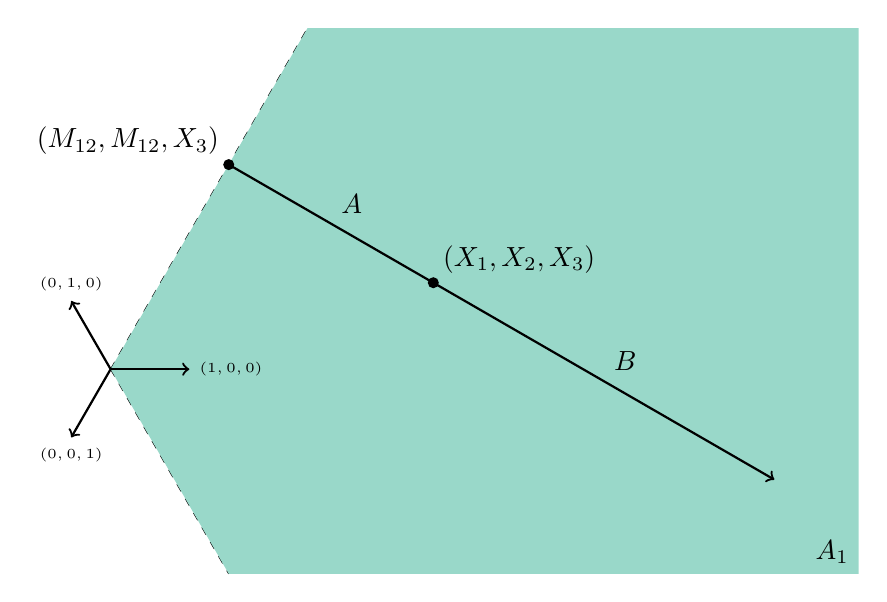
\begin{tikzpicture}
	\coordinate (C1) at (60:5);
	\coordinate (C2) at (300:3);
	\coordinate (A) at (60:3);
	\coordinate (B) at ($(A) + (330:3)$);
	\draw[dashed] (0, 0) -- (C1);
	\draw[dashed] (0, 0) -- (C2);
	\fill[mid_green] (0, 0) -- (C1) -- ($(C1) + (7, 0)$) -- ($(C2) + (8, 0)$) -- (C2) -- cycle;
	\node[above left] at ($(C2) + (8, 0)$) {$A_1$};
	\draw[thick] (A) -- (B) node[midway, above right] {$A$};
	\draw[thick, ->] (B) -- ++(330:5) node[midway, above right] {$B$};
	\fill (A) circle(2pt) node[above left] {$\left(M_{12}, M_{12}, X_3\right)$};
	\fill (B) circle(2pt) node[above right] {$\left(X_1, X_2, X_3\right)$};
	\draw[thick, ->] (0, 0) -- (1, 0) node[right] {\tiny $\left(1, 0, 0\right)$};
	\draw[thick, ->] (0, 0) -- (120:1) node[above] {\tiny $\left(0, 1, 0\right)$};
	\draw[thick, ->] (0, 0) -- (240:1) node[below] {\tiny $\left(0, 0, 1\right)$};
\end{tikzpicture}
\end{center}
\caption{The $p$-value $p_{12}$ can be written in terms of integral $A$ along the segment and $B$ along the ray. The diagram is drawn a level set of $x_1 + x_2 + x_3$. The green region represents the selection event $A_1$.}
\label{fig:p-value}
\end{figure}

\Cref{fig:compare_rays} has both the $p$-values shown on the same diagram. Proving $p_{12} \ge p_{13}$ is the same as proving
$$\frac{B}{A+B} \ge \frac{D}{C+D} ~~~~ \Longleftrightarrow ~~~~ \frac{B}{A} \ge \frac{D}{C}.$$
We will prove so by extending $A$ to include $\tilde{A}$ on the diagram. We denote the sum $A + \tilde{A}$ as $A'$. Formally,
\begin{equation}
A' = \int_{-D_{13}}^0 g\left(X_1 + z, X_2 - z, X_3\right) \,dz \ge \int_{-D_{12}}^0 g\left(X_1 + z, X_2 - z, X_3\right) \,dz = A.
\label{eqn:int_extension}
\end{equation}
It is thus sufficient to show that $B \ge D$ and $C \ge A'$.

\begin{figure}[htbp]
\begin{center}
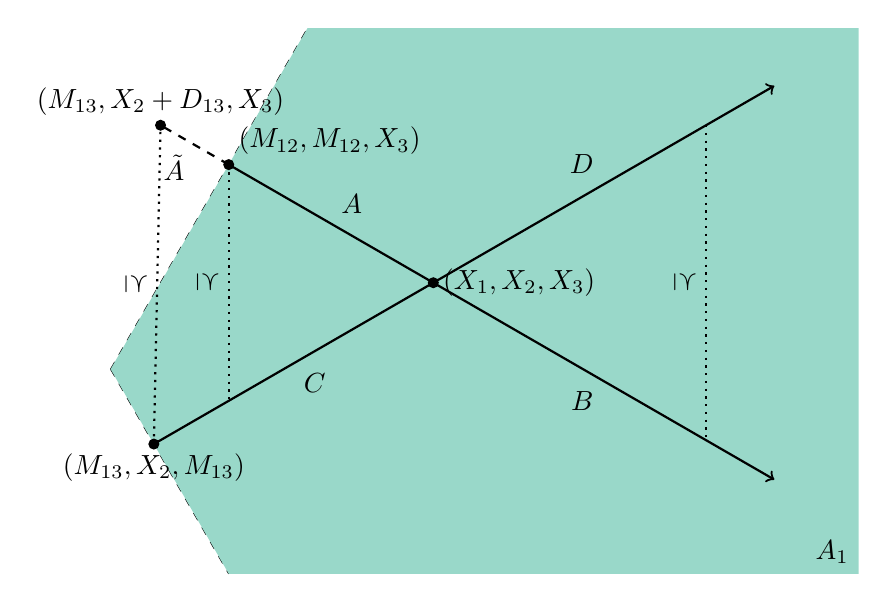
\begin{tikzpicture}
	\coordinate (C1) at (60:5);
	\coordinate (C2) at (300:3);
	\coordinate (A) at (60:3);
	\coordinate (B) at ($(A) + (330:3)$);
	\coordinate (C) at ($(0, 0)!(B)!(C2)$);
	\coordinate (D) at ($(A) + (150:1)$);
	\draw[dashed] (0, 0) -- (C1);
	\draw[dashed] (0, 0) -- (C2);
	\fill[mid_green] (0, 0) -- (C1) -- ($(C1) + (7, 0)$) -- ($(C2) + (8, 0)$) -- (C2) -- cycle;
	\node[above left] at ($(C2) + (8, 0)$) {$A_1$};
	\draw[thick] (A) -- (B) node[midway, above right] {$A$};
	\draw[thick, ->] (B) -- ++(330:5) node[midway, below left] {$B$};
	\fill (A) circle(2pt) node[above right] {$\left(M_{12}, M_{12}, X_3\right)$};
	\fill (B) circle(2pt) node[right] {$\left(X_1, X_2, X_3\right)$};
	\draw[thick] (C) -- (B) node[midway, below right] {$C$};
	\node[below] at (C) {$\left(M_{13}, X_2, M_{13}\right)$};
	\draw[thick, ->] (B) -- ++(30:5) node[midway, above left] {$D$};
	\fill ($(0, 0)!(B)!(C2)$) circle(2pt);
	\draw[thick, dashed] (A) -- (D) node[midway, below left] {$\tilde{A}$};
	\fill (D) circle(2pt) node[above] {$\left(M_{13}, X_2 + D_{13}, X_3\right)$};
	\draw[thick, dotted] (C) -- (D) node[midway, below, rotate=-90] {$\succeq$};
	\draw[thick, dotted] (A) -- ++(0, -3) node[midway, below, rotate=-90] {$\succeq$};
	\draw[thick, dotted] ($(B) + (30:4)$) -- ($(B) + (330:4)$) node[midway, below, rotate=-90] {$\succeq$};
\end{tikzpicture}
\end{center}
\caption{The $p$-value $p_{12}$ can be written in terms of integral $A$ along the segment and $B$ along the ray; and $p_{13}$ in terms of $C$ and $D$. $A'$ would refer to the sum of $A$ with the dashed line portion labeled as $\tilde{A}$, formally explained in \Cref{eqn:int_extension}. The majorization relation is indicated by the dotted line.}
\label{fig:compare_rays}
\end{figure}

Indeed from the second point \Cref{lma:two_properties} we have
$$\left(X_1 + z, X_2 - z, X_3\right) \succeq \left(X_1 + z, X_2, X_3 - z\right)$$
for $z \le 0$ and the majorization reversed for $z \ge 0$. This majorization relation is indicated as the dotted line in \Cref{fig:compare_rays}. So Schur-concavity shows that
$$g\left(X_1 + z, X_2 - z, X_3\right) \le g\left(X_1 + z, X_2, X_3 - z\right)$$
for $z \le 0$, and the inequality reversed for $z \ge 0$. Taking integrals on both sides yields the desired inequality.

For the alternative case where $X_2 \ge M_{13}$, it follows from a similar proof. In either cases, $p_{12} \ge p_{13}$, or in generality, $p_{12} \ge p_{1j}$ for $j > 1$. A test based on only $X_1$ and $X_2$ is sufficient for the null hypothesis $H_{01}$, if the carrying measure $g$ is Schur-concave. Indeed, since the denominator of $p_{12}$ under the null hypothesis, this one-sided test comparing $X_1$ and $X_2$ is identical to a naive two-sided test comparing $X_1$ and $X_2$. By \Cref{thm:stoch}, rejecting this null hypothesis is equivalent to inferring that $X_1 \ge X_j$ for all $j>1$ stochastically.

\end{proof}

As the construction of this test follows \cite{Fithian:2014ws}, it is also a uniformly most powerful unbiased selective level-$\alpha$ test.

If the distribution is discrete, the proof above holds true. Instead of performing integrals, the atoms on the rays will be summed. If ties are broken independently and randomly, as in \Cref{sec:multinomial_example}, the end points on the rays can be considered as ``half an atom''.

\section{Selective confidence bound}
\label{sec:selective_confidence_bound}

We can take the idea above further and construct confidence bound for $\theta_1 - \max_{j>1} \theta_j$. This can be achieved by considering a statistical test, to see if $\theta_1 - \max_{j>1} \theta_j \le \delta$, followed by the duality of confidence interval and statistical test.

\begin{theorem}
In the same setup as \Cref{thm:main_result}, there is a selective level-$\alpha$ lower confidence bound for $\theta_{j^*} - \max_{j \ne j^*} \theta_j$.
\end{theorem}

\begin{proof}

Again we start with assuming $X_1 \ge \cdots \ge X_n$. The null hypothesis $H_{01}^\delta$ can be thought of as $\bigcup_{j > 1} H_{01j}^\delta$, where $H_{01j}^\delta$ is $\theta_1 - \theta_j \le \delta$. In other words, we focus on the conditional law
$$\mathcal{L}_{\theta_1 - \theta_j = \delta} \left(D_{1j} \middle| D_{1j}, X_2, \ldots, X_n, A\right),$$
which is the truncated distribution
\begin{align*}
D_{1j} & \sim \exp\left(\left(\theta_1 - \theta_j\right) D_{1j} + \theta_2 X_2 + \cdots + \left(\theta_1 + \theta_j\right) M_{1j} + \cdots + \theta_n X_n \right) \\
& ~~~~~~~~ g\left(M_{ij} + D_{ij}, X_2, \ldots, M_{ij} - D_{ij}, \ldots X_n\right) 1_{A_1} \\
& \sim \exp\left(\delta D_{ij}\right) g\left(M_{ij} + D_{ij}, X_2, \ldots, M_{ij} - D_{ij}, \ldots X_n\right) 1_{A_1}.
\end{align*}

The $p$-values thus are
$$p_{1j} = \frac{\int_{D_{1j}}^\infty \exp\left(\delta z\right) g\left(M_{1j} + z, X_2, \ldots, M_{1j} - z, \ldots, X_n\right) \,dz}{\int_{\max\left\{X_2 - M_{1j}, 0\right\}}^\infty \exp\left(\delta z\right) g\left(M_{1j} + z, X_2, \ldots, M_{1j} - z, \ldots, X_n\right) \,dz}.$$

As before in \Cref{sec:exponential_families}, without loss of generality we assume $n = 3$. Once again it is sufficient to show that $p_{12} \ge p_{13}$. We have the same two cases. If $X_2 < M_{13}$, then
\begin{align*}
p_{12} & = \frac{\int_0^\infty \exp\left(\delta \left(z + D_{12}\right)\right) g\left(X_1 + z, X_2 - z, X_3\right) \,dz}{\int_{-D_{12}}^\infty \exp\left(\delta \left(z + D_{12}\right)\right) g\left(X_1 + z, X_2 - z, X_3\right) \,dz} \\
& \ge \frac{\int_0^\infty \exp\left(\delta z\right) g\left(X_1 + z, X_2 - z, X_3\right) \,dz}{\int_{-D_{13}}^\infty \exp\left(\delta z\right) g\left(X_1 + z, X_2 - z, X_3\right) \,dz} \\
p_{13} & = \frac{\int_0^\infty \exp\left(\delta \left(z + D_{13}\right)\right) g\left(X_1 + z, X_2, X_3 - z\right) \,dz}{\int_{-D_{13}}^\infty \exp\left(\delta \left(z + D_{13}\right)\right) g\left(X_1 + z, X_2, X_3 - z\right) \,dz} \\
& = \frac{\int_0^\infty \exp\left(\delta z\right) g\left(X_1 + z, X_2, X_3 - z\right) \,dz}{\int_{-D_{13}}^\infty \exp\left(\delta z\right) g\left(X_1 + z, X_2, X_3 - z\right) \,dz}
\end{align*}

The same argument in \Cref{fig:compare_rays} shows that $p_{12} \ge p_{13}$. This is again true for the case where $X_2 \ge M_{13}$ as well. This means that the bound can be constructed considering only $p_{12}$.

\end{proof}

\section{Step down procedure}
\label{sec:step_down_procedure}

If one is interested in verifying more than just the ``winner'', this selective test can also be extended to a step-down procedure that verifies the ``first runner-up'' and ``second runner-up'' etc., while controlling the FWER and the FDR.

Formally, we wish to find the biggest $j$ such that we can infer
$$\theta_1 > \ldots > \theta_j > \max_{k>j} \theta_k.$$
If $j_0$ is the true value of $j$, the two error rates we mentioned above refer to
$$\text{FWER} = \PP\left(j \ne j_0\right) ~~~~ \text{ and } ~~~~ \text{FDR} = \EE\left[\frac{\left(j - j_0\right)_+}{j}\right],$$
where $\left(j - j_0\right)_+ / j$ is taken to be $0$ if $j = 0$.

\begin{theorem}
There is a step-down procedure that infers $j_0$ above with both the FWER and FDR controlled at $\alpha$.
\end{theorem}

\begin{proof}

This can be fitted into the selective sequential model selection framework proposed by Fithian, Taylor and Tibshirani \cite{Fithian:2015uj}. Given the observations $X_1 \ge \cdots \ge X_n$, drawn from an unknown distribution $F$, we consider the sequence of null hypothesis of
$$H_{0j}: \theta_j \le \max_{k > j} \theta_k.$$
Alternatively, we can think of them as a sequence of nested model
$$M_0\left(X\right) \subseteq M_1\left(X\right) \subseteq \cdots \subseteq M_n\left(X\right), ~~~~~~~~ M_j\left(X\right)^c = \left\{\theta_1 > \cdots > \theta_j > \max_{k > j} \theta_k\right\},$$
and the each $M_j$ depends on $X$ through the order of $X$. The step-down procedure for rejecting $H_{0j}$ is equivalent to selecting the smallest $j$ for which $F \in M_j\left(X\right)$.

We can construct selective $p$-values by conditioning on $M_j\left(X\right)$, as well as other nuisance parameters. Specifically, we are conditioning on the selection of the model $M_j\left(X\right)$. We can take $p_j$ to be the survival function of the conditional law
\begin{align}
&~ \mathcal{L}_{\theta_j = \theta_{j+1}} \left(D_{j\left(j+1\right)} \middle| M_j\left(X\right), X_1, \ldots, X_{j-1}, M_{j\left(j+1\right)}, X_{j+2}, \ldots, X_n\right) \nonumber \\
= &~ \mathcal{L}_{\theta_j = \theta_{j+1}} \left(D_{j\left(j+1\right)} \middle| \left\{X_1 > \ldots > X_j > \max_{k > j} X_k\right\}, X_1, \ldots, X_{j-1}, M_{j\left(j+1\right)}, X_{j+2}, \ldots, X_n\right) \nonumber \\
= &~ \mathcal{L}_{\theta_j = \theta_{j+1}} \left(D_{j\left(j+1\right)} \middle| \left\{X_{j-1} > X_j > M_{j\left(j+1\right)}\right\}, X_1, \ldots, X_{j-1}, M_{j\left(j+1\right)}, X_{j+2}, \ldots, X_n\right). \label{eqn:step_down_law}
\end{align}

\begin{figure}[htbp]
\begin{center}
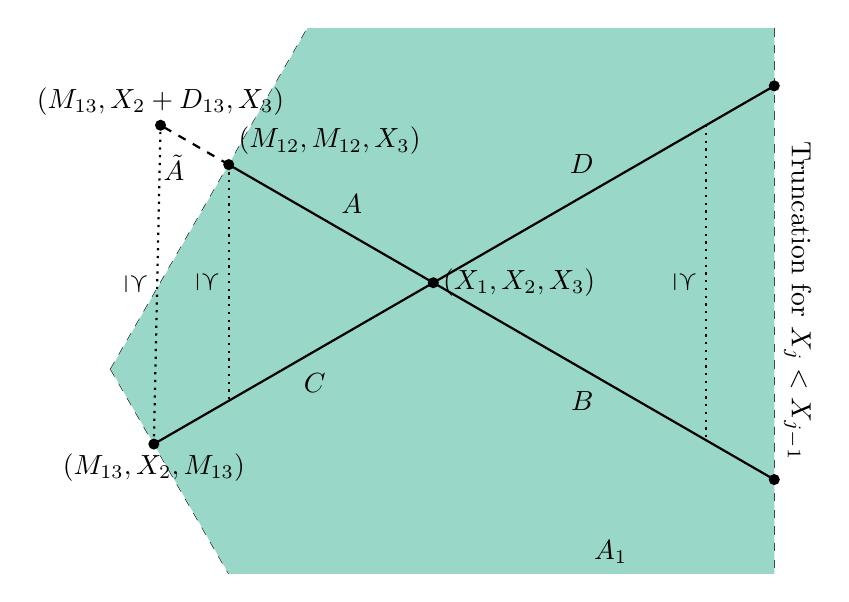
\begin{tikzpicture}
	\coordinate (C1) at (60:5);
	\coordinate (C2) at (300:3);
	\coordinate (A) at (60:3);
	\coordinate (B) at ($(A) + (330:3)$);
	\coordinate (C) at ($(0, 0)!(B)!(C2)$);
	\coordinate (D) at ($(A) + (150:1)$);
	\coordinate (C3) at ($(B) + (330:5)$);
	\coordinate (C4) at ($(B) + (30:5)$);
	\coordinate (C5) at ($(C3)!(C1)!(C4)$);
	\coordinate (C6) at ($(C3)!(C2)!(C4)$);
	\draw[dashed] (0, 0) -- (C1);
	\draw[dashed] (0, 0) -- (C2);
	\draw[dashed] (C5) -- (C6) node[midway, above, rotate = -90] {Truncation for $X_j < X_{j-1}$};
	\fill[mid_green] (0, 0) -- (C1) -- (C5) -- (C6) -- (C2) -- cycle;
	\node[above] at ($(C2)!0.7!(C6)$) {$A_1$};
	\draw[thick] (A) -- (B) node[midway, above right] {$A$};
	\draw[thick] (B) -- (C3) node[midway, below left] {$B$};
	\fill (C3) circle(2pt);
	\fill (A) circle(2pt) node[above right] {$\left(M_{12}, M_{12}, X_3\right)$};
	\fill (B) circle(2pt) node[right] {$\left(X_1, X_2, X_3\right)$};
	\draw[thick] (C) -- (B) node[midway, below right] {$C$};
	\node[below] at (C) {$\left(M_{13}, X_2, M_{13}\right)$};
	\draw[thick] (B) -- (C4) node[midway, above left] {$D$};
	\fill (C4) circle(2pt);
	\fill ($(0, 0)!(B)!(C2)$) circle(2pt);
	\draw[thick, dashed] (A) -- (D) node[midway, below left] {$\tilde{A}$};
	\fill (D) circle(2pt) node[above] {$\left(M_{13}, X_2 + D_{13}, X_3\right)$};
	\draw[thick, dotted] (C) -- (D) node[midway, below, rotate=-90] {$\succeq$};
	\draw[thick, dotted] (A) -- ++(0, -3) node[midway, below, rotate=-90] {$\succeq$};
	\draw[thick, dotted] ($(B) + (30:4)$) -- ($(B) + (330:4)$) node[midway, below, rotate=-90] {$\succeq$};
\end{tikzpicture}
\end{center}
\caption{The two $p$-values constructed corresponds to taking integrals of $g$ along these segments, that lie on a level set of $x_j + x_{j+1} + x_k$. The dashed line corresponds to extension in \Cref{eqn:int_extension}. The dotted line on the far right is the truncation that enforces $X_j < X_{j-1}$.}
\label{fig:crop_rays}
\end{figure}

Here we are only comparing $X_j$ to $X_{j+1}$ by \Cref{sec:exponential_families}. The upper truncation for $X_j$ can be represented by cropping \Cref{fig:compare_rays} along a vertical line, shown in \Cref{fig:crop_rays}, thus the proof of \Cref{thm:main_result} on sufficiency to compare $X_1$ and $X_2$ remains valid with appropriate conditioning. Again we can construct the $p$-values as in \Cref{eqn:p1j} for $k>j$.

$$p_{jk} = \frac{\int_{D_{jk}}^{X_{j-1}} g\left(X_1, \ldots, M_{jk} + z, \ldots, M_{jk} - z, \ldots, X_n\right) \,dz}{\int_{\max\left\{X_{j+1} - M_{jk}, 0\right\}}^{X_{j-1}} g\left(X_1, \ldots, M_{jk} + z, \ldots, M_{jk} - z, \ldots, X_n\right) \,dz}.$$

Hence similar to the proof of \Cref{thm:main_result}, Schur-concavity ensures $p_{j\left(j+1\right)} \ge p_{jk}$ for all $k>j$, meaning that it is sufficient to compare $X_j$ and $X_{j+1}$. In fact, we can take $p_j = p_{j\left(j+1\right)}$. These are valid selective $p$-value as required in Fithian, Taylor and Tibshirani, as
$$\PP_F \left(p_j \le \alpha \middle| M_{j-1}\left(X\right)\right) \le \alpha \text{ a.s.}, ~~~~~~~~ F \in M_{j-1}\left(X\right)$$
by tower property.

The conditioning above indeed holds some significance. The sufficient filtration \cite{Fithian:2015uj} $\mathscr{F}_k$ is given as the $\sigma$-field
\begin{align*}
\mathscr{F}_k & = \sigma\left(M_0\left(X\right), \ldots, M_j\left(X\right), X_1, \ldots, X_{j-1}, \frac{X_j + X_{j+1}}{2}, X_{j+2}, \ldots, X_n\right) \\
& = \sigma\left(\left\{X_1 > \ldots > X_j > \max_{k>j} X_k\right\}, X_1, \ldots, X_{j-1}, \frac{X_j + X_{j+1}}{2}, X_{j+2}, \ldots, X_n\right) \\
& = \sigma\left(M_j\left(X\right), X_1, \ldots, X_{j-1}, \frac{X_j + X_{j+1}}{2}, X_{j+2}, \ldots, X_n\right),
\end{align*}
which is the conditioning we used just now. Hence the nested sequence of model satisfies the subpath sufficiency principle, and the $p$-values sequence $p_j$ is independent on nulls, as defined in and shown in Theorem 4 of \cite{Fithian:2015uj}. Thus the step-down procedure where we keep rejecting $H_{0j}$ until the first time that $p_j > \alpha$ controls FWER and FDR.

\end{proof}

\section{Applications}
\label{sec:applications}

Our result above applies to a wide range of joint distributions. Note that since multiplying $-1$ preserves the majorization partial order, the following examples also work in verifying the minimum.

\begin{enumerate}

\item Correlated Gaussian: Suppose $X \sim N\left(\mu, \Sigma\right)$, where
\begin{align*}
\mu & = \left(\mu_1, \ldots, \mu_n\right), \\
\Sigma & = \begin{pmatrix}
1 & p & \cdots & p \\
p & 1 & \ddots & \vdots \\
\vdots & \ddots & \ddots & p \\
p & \cdots & p & 1
\end{pmatrix}
\end{align*}
and $p$ is fixed. Then the natural parameter is ordered the same way as $\mu$. Our test can thus be used to verify the order of the mean.

\item Multinomial distribution, e.g.\ the Iowa Republican poll example in \Cref{sec:introduction}.
$$p\left(x\right) \propto \exp\left(x^T \left(\log \pi\right)\right) \frac{1_{\left\{x_1 + \cdots + x_n = m\right\}}}{x_1! \cdots x_n!}$$
Comparing $\pi_i$ is the same as comparing $\log \pi_i$, the natural parameters. Note that the multinomial coefficient is naturally Schur-concave. The step-down procedure is applied to verify the position of the other candidates. Note that for a multinomial distribution, the conditioning \Cref{eqn:step_down_law} is equivalent to conditioning only on $M_{j\left(j+1\right)}$. We summarize the test in \Cref{tbl:poll_analysis}.

\begin{table}[htbp]
\begin{center}
\begin{tabular}{c c c c c}
\hline
Rank ($j$) & $X_{j-1}$ & $X_j$ & $X_{j+1}$ & $p$-value \\
\hline
$1$ & $\infty$ & $276$ & $214$ & $0.0065$ \\
$2$ & $276$ & $214$ & $151$ & $0.0015$ \\
$3$ & $214$ & $151$ & $71$ & $1.1126 \times 10^{-7}$ \\
$4$ & $151$ & $71$ & $36$ & $0.0014$ \\
$5$ & $71$ & $36$ & $36$ & $1.0000$ \\
\hline
\end{tabular}
\end{center}
\caption{Applying the step-down procedure to the Iowa Republican caucus. Each $p$-value is constructed by considering the conditional law in \Cref{eqn:step_down_law}, a $\text{Binomial}\left(X_j + X_{j-1}, \frac{1}{2}\right)$ truncated at $X_{j-1}$. The result was also indicated in \Cref{tbl:poll}.}
\label{tbl:poll_analysis}
\end{table}

We can also construct selective confidence bound for $\log \pi_1 - \max_{j>1} \log \pi_j$, i.e.\ find a $\delta^*$ such that
$$\PP_{H_{01}^\delta} \left(\text{reject } H_{01}^\delta: \log \pi_1 - \max_{j>1} \log \pi_j \le \delta \middle| A_1\right) < 0.05,$$
according to \Cref{sec:selective_confidence_bound}.

Once again, for multinomial distribution, conditioning on $M_{12}, X_3, \ldots, X_n$ is the same as conditioning on $M_{12}$, which gives $X_1 \sim \text{Binomial}\left(X_1 + X_2, \frac{e^\delta}{e^\delta + 1}\right)$, truncated at $M_{12}$. There is a maximum $\delta^*$ for this truncated binomial distribution has a survival function of $0.05$ at $X_1$.

This gives $\delta^* = 0.103142$. This translates to $\log \pi_1 - \max_{j>1} \log \pi_j \ge 0.103142$, or $\pi_1 / \max_{j>1} \pi_j \ge 1.10865$, with $0.95$-confidence. Or in terms of the Iowa Republican poll example, Trump has relatively around $11\%$ more support than any other candidates. This is smaller than the number deduced from raw vote count, $\left(276 - 214\right) / 214 \approx 29\%$, accounting for selection bias.

\item Independent binomials
$$p\left(x\right) \propto \exp\left(x^T \left(\log p\right)\right) \frac{1}{x_1! \left(m-x_1\right)! \cdots x_n! \left(m-p_x\right)!}$$

\item Round robin tournaments with the Bradley--Terry model, where each player has a score $\theta_i$, and the probability of player $j$ winning against player $k$ is
$$\frac{e^{\theta_j - \theta_k}}{1 + e^{\theta_j - \theta_k}} = \frac{e^{\left(\theta_j - \theta_k\right) / 2}}{e^{\left(\theta_j - \theta_k\right) / 2} + e^{\left(\theta_k - \theta_j\right) / 2}}.$$

Suppose $Y_{jk} = 1$ if $j$ beats $k$ and $Y_{jk} = 0$ if $k$ beats $j$. We will also adopt the convention that $Y_{jk} + Y_{kj} = 1$. Thus the joint distribution of $\left(Y_{jk}\right)_{j, k}$ is
$$p\left(\left(y_{jk}\right)_{j, k}\right) \propto \exp\left(\sum_j 2\theta_j \sum_{k \ne j} y_{jk}\right)  = \exp\left(\theta^T x\right),$$
where $x_j = \sum_{k \ne j} y_{jk}$. In other words, $x_j$ is the number of wins by player $j$.

If the individual results are masked and we only know about the net wins, then
$$p\left(x\right) \propto \exp\left(2\theta^T x\right) g\left(x\right),$$
where $g\left(x\right)$ is a function that count number of possible tournament results giving the net win vector $x$. A bijection proof shows that $x$ is indeed Schur-concave, allowing to apply the main result in comparing $2\theta$ and thus $\theta$.

\end{enumerate}

\bibliographystyle{plainnat}
\bibliography{papers,additional}

\end{document}